\chapter {Media}

Ne gândim la media ca mijloace de comunicare în primul rând: presa, radioul și televiziunea.
Marshall McLuhan, cel care a pus bazele studiului teoriei media, se gândește la mediu ca la o extensie a corpului sau a minții umane: hainele prelungesc pielea, casa prelungește mecanismul de reglare a temperaturii corpului, bicicleta și automobilul sunt extensii ale piciorului. Un mediu sau o tehnologie poate fi orice extensie a corpului uman.

Formele media se pot cuprinde unele pe altele, astfel telegraful conține cuvântul tipărit, care conține scrisul, care la rândul său, conține vorbirea. Mediul conținut este mesajul mediului care îl conține. Dar nu toate formele media acționează în pereche. McLuhan identifică niște excepții, cea mai notabilă fiind gândul ca proces non-verbal și pur.

Pentru a utiliza media în mod eficient, efectele acesteia trebuiesc studiate, fiindcă reprezintă niște factori importanți în modul în care ne folosim simțurile și în care interacționăm atât între noi cât și cu ecosistemul ce se îndreaptă cu efect de bulgăre în sfera cyberpunk-ului.

În cartea sa, \textit{Să înțelegem Media}, McLuhan revine mereu asupra ideii că \textit{„Mediul este mesajul”}.
Pentru a clarifica această idee, un exemplu simplu ar fi lumina electrică. Este irelevant dacă lumina este utilizată în neurochirurgie sau la un meci de fotbal în nocturnă. S-ar putea argumenta ca aceste activități sunt „conținutul” luminii electrice, din moment ce ele nu ar putea exista fără lumina electrică.
În acest sens: \begin{quotation}
„Mediul este mesajul” deoarece mediul este cel care modelează și controlează dimensiunea și forma acțiunii sau asocierii umane.
\end{quotation}

\section{Constrângeri}

Actorul Prince Modupe scria în autobiografia sa despre contactul său cu efectele cuvântului vorbit în vremurile în care trăia în Africa de Vest:
\begin{quote}
Singurul spațiu aglomerat din casa părintelui Perry erau rafturile sale cu cărți. Cu vremea, am ajuns să înțeleg că semnele de pe pagini erau \textit{cuvinte prinse în capcană}. Oricine putea învăța sa descifreze simbolurile și să prefacă la loc în vorbire cuvintele prinse în capcană. Cerneala tiparului ținea gândurile captive; ele nu puteau scăpa de acolo mai mult decât putea un \textit{elefant} să iasă dintr-un puț. Când revelația însemnătății acestui lucru s-a revărsat asupra mea, am simțit același fior și aceeași uimire ca atunci când am văzut prima dată luminile strălucitoare din Konakry. Tremuram de dorința intensă de a învăța să fac eu însumi acest lucru uimitor.
\end{quote}

Gândul este proces non-verbal și pur. Este mediul primar care, urmând ideii lui McLuhen, este rădăcina arborelui extensiilor umane. Are ca extensie corpul, cu toate simțurile lui, vorbirea ca mijloc principal de exprimare și tehnologia informației ca mediu de stocare și procesare.

Fiecare nod din ceastă entitate complexă comunică cu extensiile ei prin diferite moduri, între cele naturale (gând - membre, gând - vorbit) comunicare se face prin sistemul nervos central și se produce instantaneu. Comunicarea cu extensiile oferite de tehnologie se face printr-o interfață concepută de noi (pedalele unei biciclete, întrerupătorul unui bec, ecranul unui telefon mobil). Aceste interfețe reprezintă în acest moment cele mai mari constrângeri ale folosirii eficiente a acestor unelte.

\section{Concepte}

A.N. Whitehead a explicat că cea mai mare descoperire a secolului XX a fost descoperirea tehnicii de descoperire. Adică tehnica de a începe cu lucrul care trebuie descoperit și apoi de a merge înapoi, pas cu pas, ca pe o linie de montaj, până la punctul în care este necesar să se reînceapă pentru a ajunge la obiectul dorit. 
În artă, aceasta înseamnă să începi cu \textit{efectul} și apoi să inventezi un poem, un tablou sau o clădire care să aibă exact efectul în cauză și nu altul.\\

ENIAC\footnote{Prescurtare de la Electronic Numerical Integrator And Computer (Calculator și Integrator Electronic Numeric).} a fost primul calculator electronic de uz general. Era un calculator numeric (digital), Turing-complet, capabil de a fi reprogramat pentru a rezolva o gamă largă de probleme calculatorii.
Era uriaș, costa cam o jumătate de milion de dolari la vremea respectivă, cântărind aproape 30 de tone și avea nevoie de mai multe persoane pentru a fi operat. Odată cu introducerea acestuia în 1946 putem spune că a apărut computerul ca tehnologie. \\

\begin{figure}[h]
  \centering
  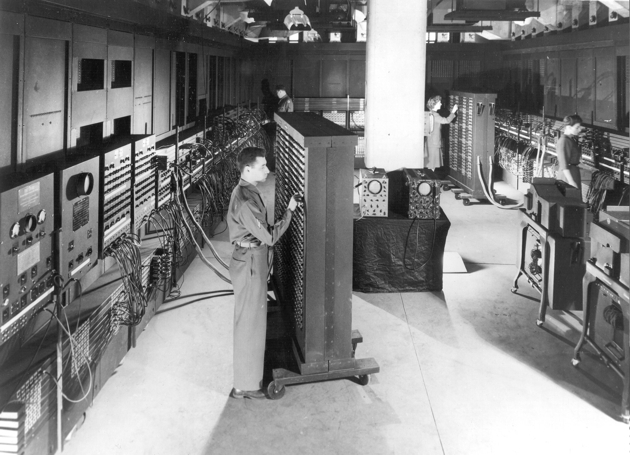
\includegraphics[scale=0.8]{img/eniac.jpg}
  \caption{Cap. Herman Goldstein (în faţă) setează comutatoarele unuia dintre tablourile funcţionale ale ENIAC la Şcoala Moore de Inginerie Electrică. (foto: Armata SUA)}
\end{figure}
\newpage

Transformarea acestuia în mediu a început însă mai târziu. Douglas Engelbart, unul dintre cei care a pus bazele computerelor personale și-a prezentat viziunea de a augmenta inteligența umană cu ajutorul computerelor.

În 1968 Engelbart a prezentat prototipul viziunii sale, numit NLS\footnote{Un sistem complet hardware și software, prescurtare de la "the oN-Line System", }.
Această prezentarea ajuns mai târziu să fie supranumită \textit{Mama tuturor demonstrațiilor}\footnote{În original „Mother of all demos”} deoarece a introdus foarte multe concepte pe care le folosim și astăzi; mouse-ul, ferestrele, interfața grafică, video-conferința, procesarea text, hipertextul, versionarea sau editorul colaborativ în timp real.

Câțiva ani mai târziu Alan Kay a prezentat Dynabook, un prototip al unei platforme colaborative pentru copii.
Un computer portabil cu interfață grafica și touchscreen, capabil de accesare și partajare a informațiilor în rețea. A prezentat o viziune detaliată a tabletelor cu touchscreen decenii înainte să devină practice. Dar mai mult decât o tabletă, el a conceptualizat un mediu dinamic cu care ne putem juca și interacționa.

\begin{figure}[h]
  \centering
  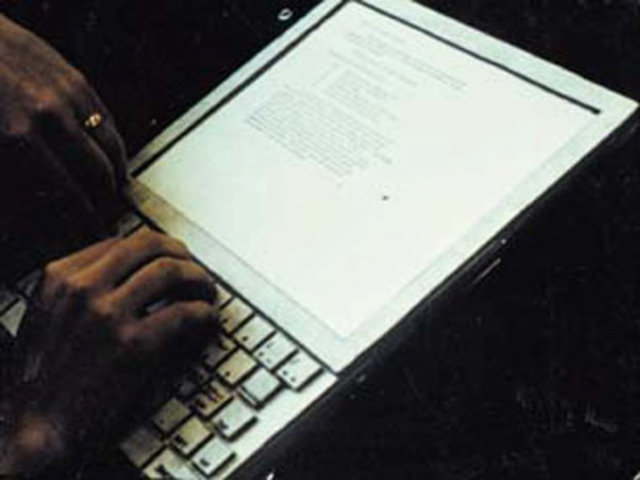
\includegraphics[scale=0.6]{img/dynabook.jpg}
  \caption{Dynabook, dezvoltat și prezentat in 1972}
\end{figure}
\newpage

Aceste concepte perfecționate de-a lungul timpului ne-au adus din ce în ce mai aproape de tehnologie. Dispozitivele electronicele au devenit omniprezente și interconectate. Le purtăm pretutindeni, le putem accesa de la distanță și le putem programa să îndeplinească sarcini în lipsa noastră.

Dar cu toate că am reușit să facem computere mai rapide, mai puternice, mai mici și mai frumoase, modul în care interacționăm cu ele are la bază aceleași concepte introduse acum câteva decenii.

\section{Soluții}

Schimbarea modului în care interacționăm cu tehnologia întâmpină o serie de obstacole de diferite grade de dificultate. Dar pentru a le depăși pe cele mai importante este nevoie de câteva lucruri.

\subsection{Asumarea riscului}

Este cunoscut faptul ca majorității oamenilor le este frica de schimbare. Atâta timp cât confortabila rutină pe care și-au stabilit-o le asigură mijloacele de subzistență, le este frică să se angajeze în ceva ce ar putea eșua, așa că nu încearcă.

Acest lucru este valabil și la nivel de companii, ieșirea din tipar reprezintă un risc prea mare dacă soluția actuală funcționează, fie și la un nivel considerabil sub-optim. Schimbări radicale sau soluții fundamental diferite luându-se în considerare fie în pragul falimentului, fie datorită unei abundențe a resurselor, când costul nu reprezintă o problemă, iar unda șocului eșecului poate fi ușor absorbită.

Asumarea riscurilor este o componentă cheie pentru transformarea în realitate a ideilor revoluționare, pentru inovație.

\subsection{Creativitate}

Procesul de îmbunătățire a tehnologiilor actuale poate fi descris printr-o serie simplă de pași: analizarea dispozitivului în cauză, observarea modului în care este utilizat, găsirea punctelor slabe și concentrarea resurselor asupra găsirii unei soluții, de cele mai multe ori similară, dar mai rapidă și mai eficientă pentru a rezolva aceeași problemă.

Găsirea unor soluții complet noi necesită ieșirea din bula conceptelor deja existente și aplicarea tehnicii de descoperire mai sus menționată.

Un exemplu ce portretizează foarte bine atât creativitatea cât și utilizarea acțiunilor naturale pentru atenuarea curbei de învățare necesar folosirii dispozitivului, este \textit{Robotul telefonic cu biluțe}\footnote{Original \textit{Marble Answering Machine}, "marble" nu are o traducere exactă, sunt biluțe din sticlă, oțel sau agat.}.

\begin{figure}[h]
  \centering
  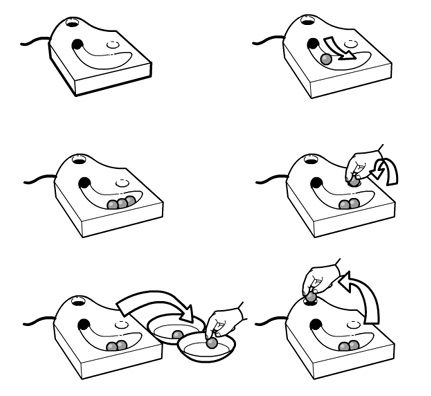
\includegraphics[scale=0.6]{img/marbleAnswMachine.png}
  \caption{Schițe reprezentând modul de utilizare al Robotului telefonic cu biluțe, propus in 1992}
\end{figure}

Robotul telefonic cu biluțe este un prototip proiectat de Durrell Bishop în 1992, și este considerat una dintre primele interfețe cu utilizatorul tangibile sau \textit{TUI}\footnote{TUI, acronim pentru "Tangible user interface"}.
Dispozitivul eliberează o biluță pentru fiecare mesaj vocal primit. Ordinea bilelor indică ordinea în care mesajele au fost recepționate. Mesajele pot fi ascultate plasând biluța corespunzătoare într-un recipient special, salvate prin păstrarea lor fizică, sau șterse prin reintroducerea lor în circuit. Scopul acestui robot telefonic era de a demonstra potențialul de a face informația digitală palpabilă.

\subsection{Uciderea mesagerului}

Comunicarea cea mai eficientă între entități se face atunci când este efectua direct, fără a fi alterată de intermediari.

În cazul interacțiunii omului cu informația digitală acest lucru se poate obține fie prin materializarea acesteia în \textit{metafore palpabile} ca în exemplul biluțelor robotului telefonic, fie prin interacțiune directă cu aceasta în mediul ei natural.
\textit{Realitatea augmentată} ne permite aducerea informației digitale nealterate în lumea reală iar \textit{realitatea virtuală} ne permite să pășim în lumea acesteia.
Dispozitive ca \textit{Leap motion} elimină necesitatea perifericelor ca tastatura, mouse-ul, touchscreen-ul sau joystick-ul, noi înșine devenind „controller-ul”.

\begin{figure}[h]
  \centering
  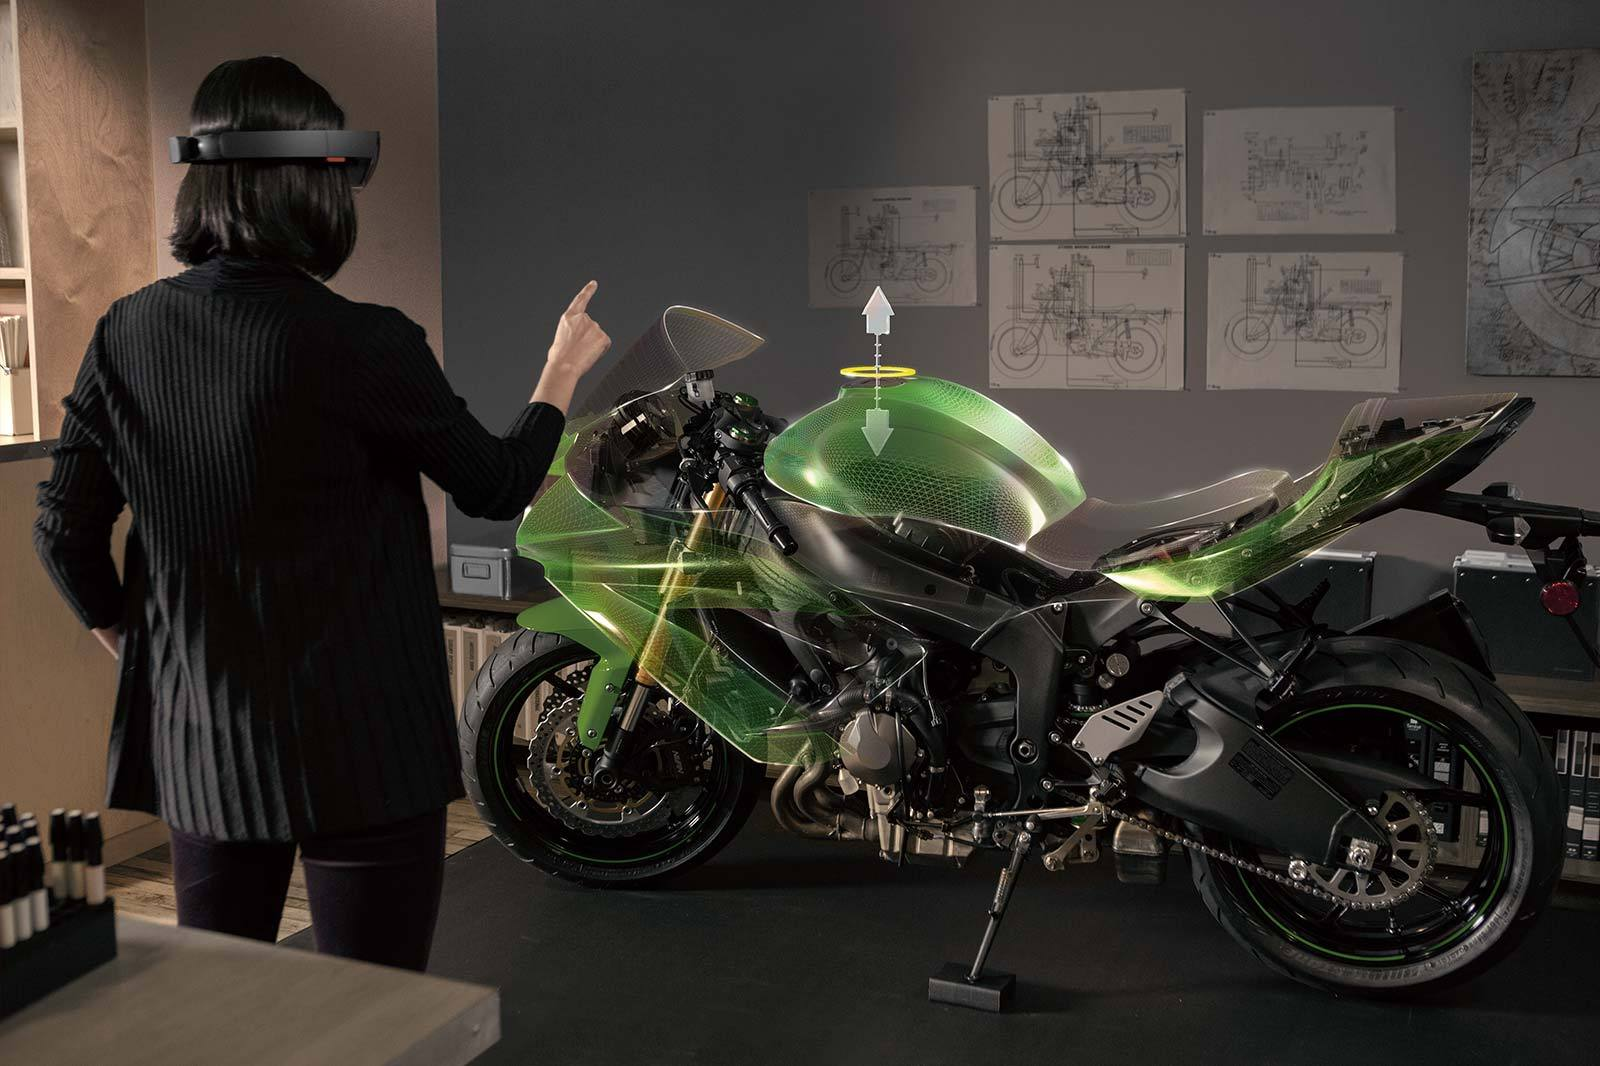
\includegraphics[scale=0.25]{img/microsoft_hololens_demo.jpg}
  \caption{Realitate augmentată, demonstrație a dispozitivului \textit{HoloLens} dezvoltat de Microsoft}
\end{figure}
